%%\documentclass[t,handout]{beamer}
\documentclass{beamer}


\usepackage[utf8]{inputenc}
\usepackage[portuguese]{babel}
\usepackage[tight]{subfigure}
\usepackage{graphicx}
\usepackage{color}
\usepackage{url}
% \usepackage{listings}
%\usepackage[alf]{abntcite}

%Pacote de listagem de c�digo
\usepackage{listings}
\lstset{numbers=left, stepnumber=1, firstnumber=1,
numberstyle=\tiny, extendedchars=true, breaklines=true, frame=tb,
basicstyle=\footnotesize, stringstyle=\ttfamily,
showstringspaces=false }


\usetheme{Frankfurt} %LEGAL     !!!
% \usetheme{Madrid}     %LEGAL/L%IMPO/COM CAIXA     (sem barra de desenvolvimento)

% \usetheme{Antibes} %NAO
% \usetheme{Berlin} %PODE SER...     (BARRA DE DESENVOLVIMANTO)
% \usetheme{Berkeley}     %FEIO
% \usetheme{Boadilla} %TUDO BRANCO...
% \usetheme{Copenhagen}     %NAO
% \usetheme{Darmstadt} %LEGAL!     !!!
% \usetheme{Dresden}     %LEGAL/LIMPO/SEM CAIXA     (sem caixa fica ruim...)

% \usetheme{Goettingen}     %FEIO DEMAIS!
%\usetheme{Ilmenau} %LEGAL (forte candidato)
% \usetheme{JuanLesPins} %BACANA
% \usetheme{Luebeck}     %FEIO

% \usetheme{Malmoe}     %FEIO
% \usetheme{Warsaw} %NAO...
% \usetheme{Seattle}
% \usetheme{CambridgeUS}
% \usetheme{Singapore}

% \usecolortheme[RGB={130,35,150}]{structure}
% \usecolortheme[RGB={33,33,94}]{structure}
\usecolortheme[RGB={134,153,188}]{structure}
\setbeamertemplate{footline}[frame number]
\setbeamertemplate{navigation symbols}{}

\author[L. Medeiros]{Aluno: Leonardo Melo de Medeiros}
\date{\today}
\institute[]{Orientador: Leandro Dias da Silva\\
						 Co-orientador: Hyggo Oliveira de Almeida \\ 
						 Universidade Federal de Campina Grande - UFCG}
    \title{Monitoramento de Dados Motores Por Intermédio de Jogos Eletrônicos}
\logo{
\includegraphics[width=0.2\linewidth]{img/logo.png}}
\subtitle{Proposta de Tese}

\begin{document}

\begin{frame}
  \titlepage
\end{frame}

% \section{Roteiro}
% \AtBeginSection[]
{\frame{
\frametitle{Roteiro}
\tableofcontents
}
}

\section{Introdução}
\subsection{}
%\subsection{Problemática}
\begin{frame}{Sistemas de Monitoramento de Saúde}
  \begin{block}{}
      \center 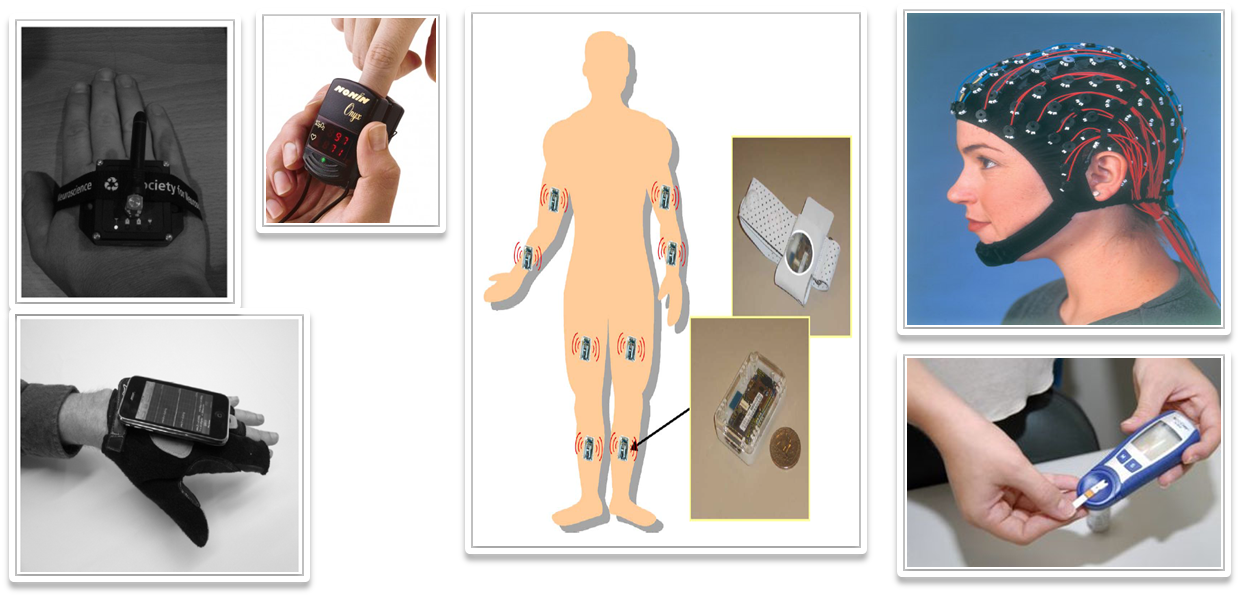
\includegraphics[height=1.8 in]{img/sismonsaude.png}
  \end{block}
  \begin{block}{}
A computação pervasiva aplicada ao contexto de saúde permite monitorar remotamente o estado de saúde dos usuários. Entretanto, a concepção de um sistema não invasivo de monitoramento é um grande desafio~\cite{alemdar}.
  \end{block}
\end{frame}

\begin{frame}{Estratégias de Monitoramento da Saúde}
  \begin{block}{}
      \center 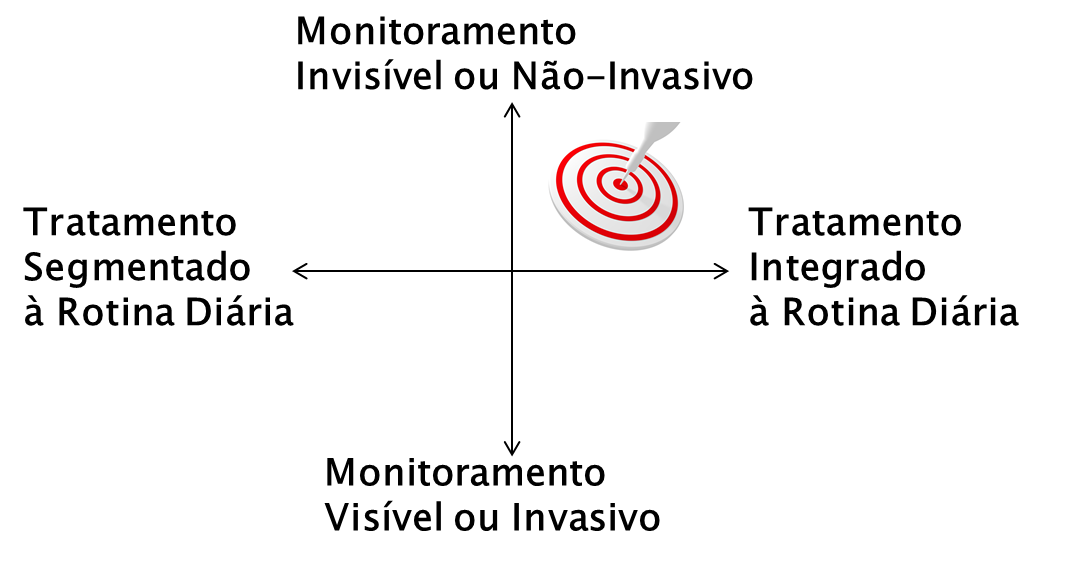
\includegraphics[height=1.8 in]{img/estrategmonitorament.png}
  \end{block}
  \begin{block}{}
As tecnologias de monitoramento para serem aceitas precisam preservar a privacidade do usuário e integrar-se à sua rotina diária~\cite{aarh10}.
  \end{block}
\end{frame}

\begin{frame}{Motivação para uso de jogos para monitoramento dos dados motores}
	\begin{block}{}
	\begin{itemize}[<+->]
			\item Percentual expressivo de adultos e idosos que são usuários de jogos, e os utiliza em sua rotina diária (29\% acima dos 50 anos);
      \item O  jogo é uma experiência autotélica, logo o usuário joga por puro prazer, sem esperar qualquer benefício por seu uso ~\cite{sweetser2005-gameflow};
			\item As tecnologias de sensores de movimento estão presentes no contexto dos jogos eletrônicos;
			\item Possibilita a reprodução de movimentos específicos em um ambiente controlado, o qual permite a aquisição de dados motores.
	\end{itemize}
	\end{block}
\end{frame}


%\subsection{Objetivos}
\begin{frame}{Objetivo Principal}
  \begin{block}{}<1->
Neste trabalho, tem-se como objetivo a concepção de uma abordagem computacional para o monitoramento de dados motores. Pretende-se usar jogos eletrônicos como forma de motivar e abstrair o monitoramento de dados de saúde de uma maneira não invasiva e longe do contexto de tratamento de saúde.
  \end{block}
\end{frame}


\begin{frame}{Hipóteses do Trabalho}
	\begin{block}{}
			\begin{itemize}[<+->]
       \item \textbf{H1} - O acompanhamento de sintomas motores, integrados à rotina diária do paciente traz benefícios ao tratamento e qualidade de vida do mesmo do ponto de vista do profissional da saúde.
       \item \textbf{H2} - É possível capturar dados motores por meio de sensores de movimento utilizados em jogos eletrônicos. Esses dados auxiliam no acompanhamento de doenças com comprometimento motor.
			\item \textbf{H3} - É possível desenvolver um jogo que tenha mecanismos de captura de dados motores embutidos, e que permita monitorar e quantificar esses dados de maneira não-invasiva.
			\end{itemize}
	\end{block}
\end{frame}

\begin{frame}{Objetivos Específicos}
	\begin{block}{}
	\begin{itemize}[<+->]
      \item Identificar a importância de realizar monitoramento de dados junto a profissionais de saúde;
			\item Usar bases de dados de saúde já consolidadas para testar abordagens de monitoramento;
			\item Identificar viabilidade técnica da aquisição de sintomas por sensores de movimento utilizados em jogos eletrônicos;
			\item Definir e implementar a arquitetura de software da abordagem;
			\item Realizar experimentos para validar as hipóteses.
	\end{itemize}
	\end{block}
\end{frame}

\section{Estudo de Caso}
\subsection{}
\begin{frame}{Doença de Parkinson}
  \begin{block}{}
    A doença de Parkinson (DP) é uma afecção do sistema nervoso central, a qual é expressa de forma crônica e progressiva. 
      \begin{itemize}[<+->]
       \item Causada pela morte dos neurônios produtores de dopamina da substância negra ~\cite{protpar010}. 
       \item Caracterizada pelos sinais cardinais de rigidez, bradicinesia, tremor e instabilidade postural ~\cite{menezes2003}.
      \end{itemize}
  \end{block}

  \begin{block}{Termos: Tremor de Repouso e Bradicinesia}<3->
      \begin{itemize}
       \item \textbf{Tremor de Repouso:} sintoma mais frequente e perceptível;
       \item \textbf{Bradicinesia:} lentidão na execução do movimento;
      \end{itemize}
  \end{block}
\end{frame}

%\subsection{Monitoramento Sintomas}
\begin{frame}{Estágios da Doença}
  \begin{block}{Escala Unificada de Avaliação da Doença de Parkinson (UPDRS)}
    A escala UPDRS ~\cite{updrs87} avalia tanto o nível de estrutura e função corporal quanto o nível das atividades.
      A escala contém itens referentes a:
	\begin{itemize}[<+->]
	 \item Mental, comportamento e humor;
	 \item atividades da vida diária;
	 \item exame motor;
	 \item complicações no tratamento.
	\end{itemize}
 \end{block}
\end{frame}

\begin{frame}{Escala (UPDRS)} 
    \begin{block}{Fenômeno (\textit{On/Off})}
      \center 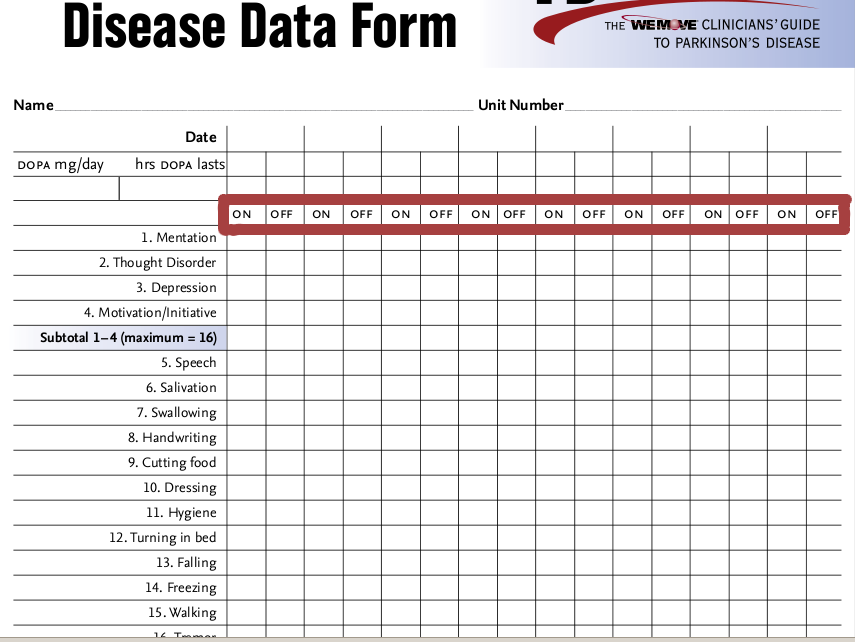
\includegraphics[height=2.4 in]{img/updr1-sel.png}
    \end{block}		
\end{frame}

\begin{frame}{Escala (UPDRS)} 
    \begin{block}{Impacto nas Atividades Diárias}
      \center 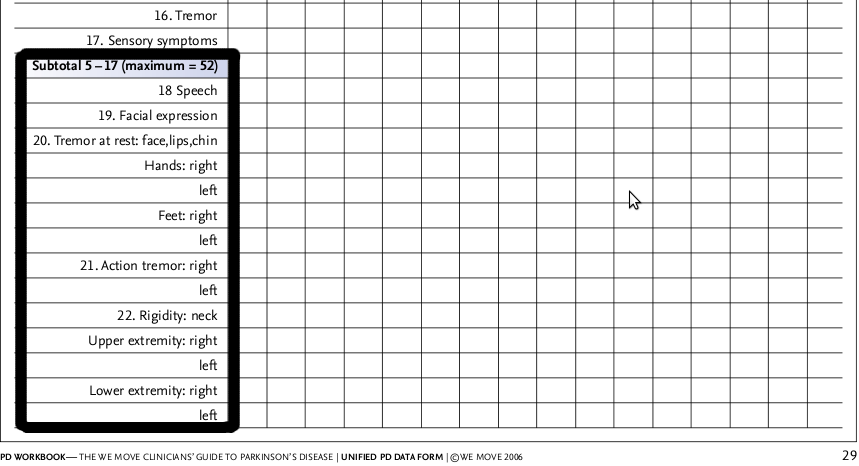
\includegraphics[height=2.0 in]{img/updr2-sel.png}
    \end{block}
\end{frame}

%\subsection{Entrevista Semi-Estruturada}
\begin{frame}{Entrevista Semi-Estruturada com Profissionais de Saúde} 
    \begin{block}{Objetivo da Pesquisa}
      Validar a Hipótese \textbf{H1}: O acompanhamento de sintomas motores, integrados à rotina diária do paciente, traz benefícios ao tratamento e qualidade de vida do mesmo, do ponto de vista do profissional da saúde.
    \end{block}
		\begin{block}{Participantes}
			\begin{table}[h]
			%\caption{Perfil dos Participantes}
			%\label{table:perfil_analise_participantes}
			\begin{tabular}{|l|l|c|c|}
			\hline
			\textbf{LEGENDA} & \textbf{PROFISSÃO}             & \multicolumn{1}{|l|}{\textbf{EXPERIÊNCIA (ANOS)}} \\ \hline
			FIS\_01          & Fisioterapeuta & 10                                                \\ \hline
			FIS\_02          & Fisioterapeuta    & 10                                                \\ \hline
			NEU\_01          & Neurologista            & 15                                                \\ \hline
			NEU\_02          & Neurologista            & 30                                                \\ \hline
			\end{tabular}
			\end{table}
    \end{block}
\end{frame} 

\begin{frame}{Resultado da Entrevista} 
    \begin{block}{}
			\begin{itemize}[<+->]
				\item Com base na rastreabilidade dos fragmentos da entrevista, pode-se concluir que existiram muitas ocorrências sobre: 
					\begin{enumerate}
						\item tremor;
						\item bradicinesia;
						\item análise da marcha.
					\end{enumerate}
				\item Para o acompanhamento e monitoramento da doença, os profissionais de saúde citaram a importância de calcular:
					\begin{enumerate}
						\item amplitude dos movimentos de abdução e adução dos braços;
						\item a velocidade angular desse movimento.
					\end{enumerate}
			\end{itemize}
    \end{block}
\end{frame} 


\section{Desenv. de Jogos}
\subsection{}


%\subsection{Jogos Para Monitoramento da Saúde}
\begin{frame}{Processo de Desenvolvimento de um Jogo para Monitoramento de Dados de Saúde}
\begin{block}{}
Este trabalho pretende usar um ambiente de jogo para a execução de movimentos específicos com o propósito de quantificar os sinais motores dos usuários e consequentemente realizar o monitoramento. 
\end{block}
\begin{block}{}
O ambiente será denominado de \textbf{GAHME}.
\end{block}
\end{frame}

%\subsection{Desenvolvimento de Jogos}
\begin{frame}{Fases de Um Processo de Desenvolvimento de Jogos}
  \begin{block}{}
      \center 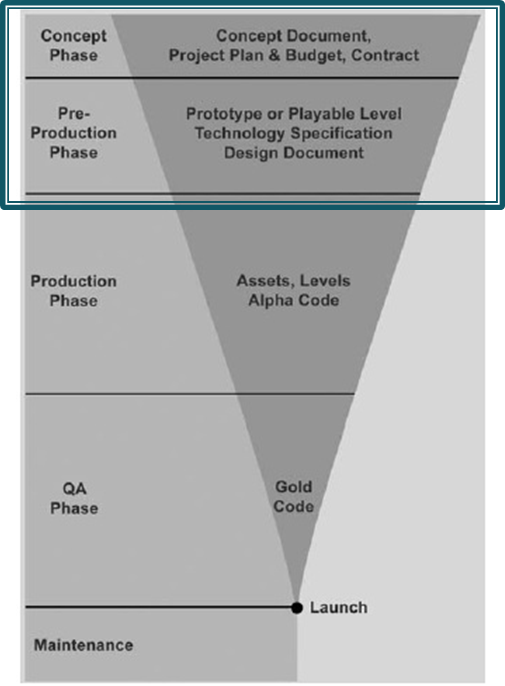
\includegraphics[height=2.8 in]{img/stages-game-development.png}
			%\caption{Modificações no Jogo ao Longo das Fases de Desenvolvimento~\cite{fullerton2008game}}
  \end{block}
\end{frame}

\begin{frame}{Fase de Conceito de um GAHME}
  %\begin{block}{}
      \center 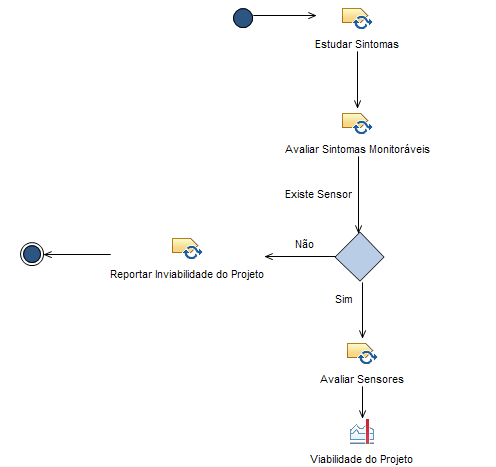
\includegraphics[height=2.8 in]{img/gahme-fase-conceito.png}
			%\caption{Modificações no Jogo ao Longo das Fases de Desenvolvimento~\cite{fullerton2008game}}
  %\end{block}
\end{frame}

\begin{frame}{Fase de Pré-Produção de um GAHME}
  %\begin{block}{}
      \center 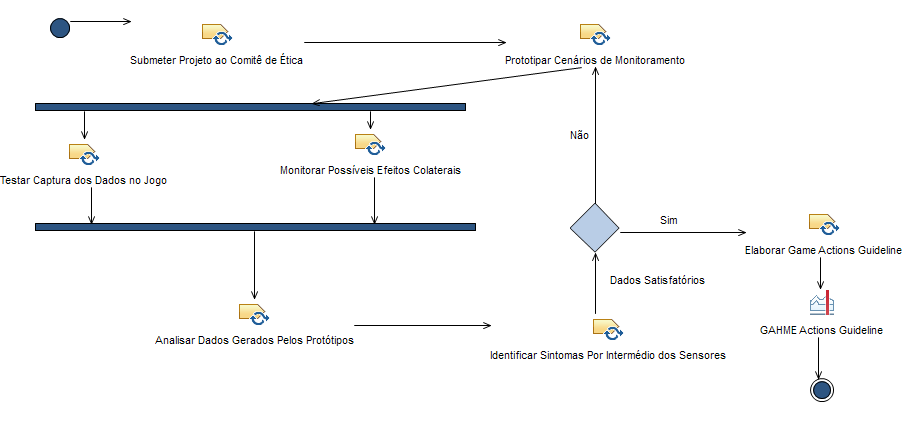
\includegraphics[height=2.1 in]{img/gahme-fase-pre-producao.png}
			%\caption{Modificações no Jogo ao Longo das Fases de Desenvolvimento~\cite{fullerton2008game}}
  %\end{block}
\end{frame}


\section{GAHME}
\subsection{}
%\subsection{Concepção}
\begin{frame}{GAHME – \textit{Health Monitor Environment}}
  %\begin{block}{}
      \top 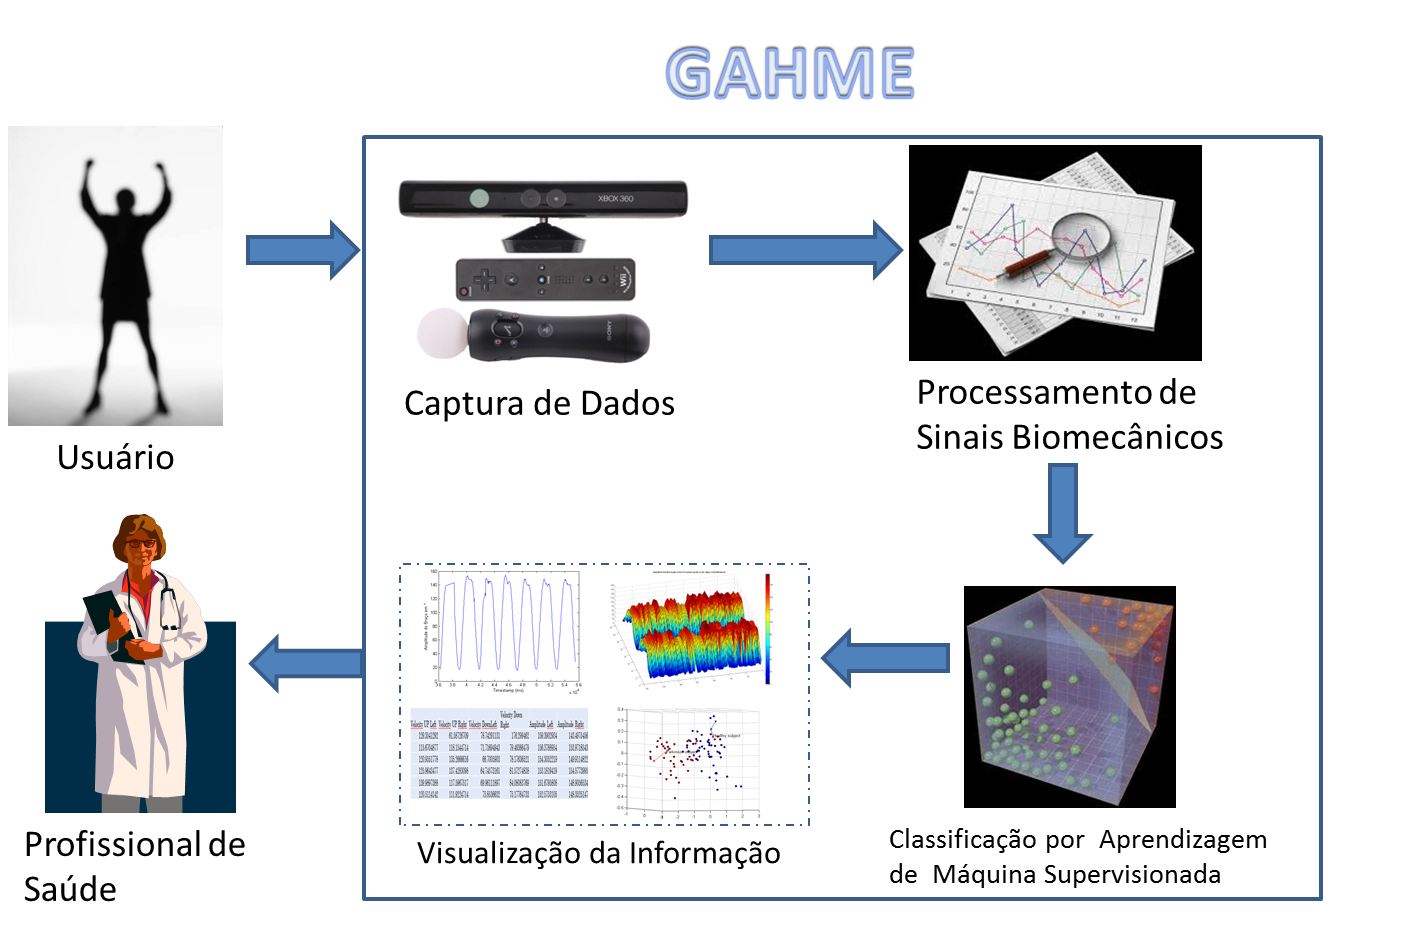
\includegraphics[height=2.6 in]{img/systemoverview.png}
			%\caption{Modificações no Jogo ao Longo das Fases de Desenvolvimento~\cite{fullerton2008game}}
  %\end{block}
\end{frame}

\begin{frame}{GAHME – \textit{Health Monitor Environment}}
	\begin{block}{}
		\begin{itemize}[<+->]
			\item	\textbf{REQ-GAHME-01} - Pontuação e Taxa de Acerto;
			\item	\textbf{REQ-GAHME-02} - Progresso e Evolução do Jogador e dos Desafios;
			\item	\textbf{REQ-GAHME-03} - Estado de Fluxo;
			\item	\textbf{REQ-GAHME-04} - Preocupação com Integridade Física do Jogador;
			\item	\textbf{REQ-GAHME-05} - Captura e Armazenamento de Sinais Motores;
			\item	\textbf{REQ-GAHME-06} - Mecanismo de Identificação de Sintomas Motores;
			\item	\textbf{REQ-GAHME-07} - Mecanismo de Visualização dos Parâmetros Motores do Usuário.
		\end{itemize}
	\end{block}
\end{frame}

\begin{frame}{Arquitetura GAHME}
  \begin{block}{}
      \center 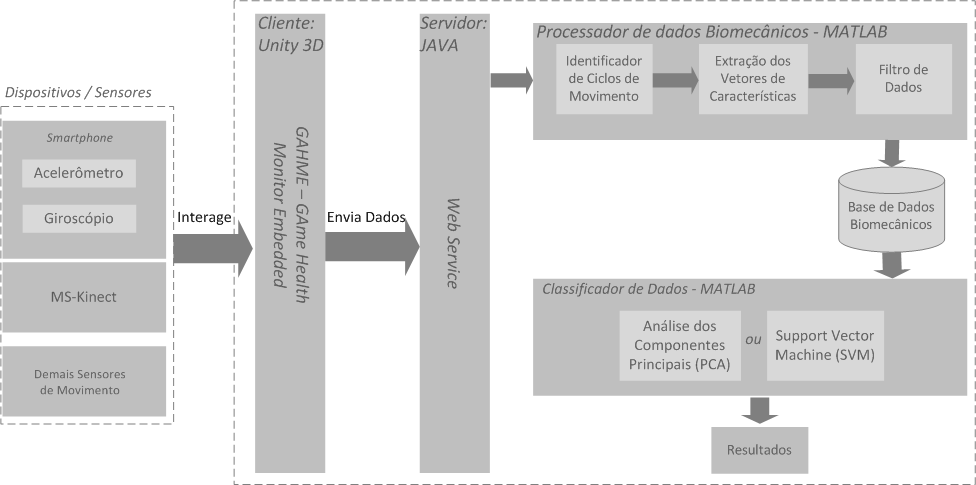
\includegraphics[height=2.0 in]{img/arquitetura.png}
			%\caption{Modificações no Jogo ao Longo das Fases de Desenvolvimento~\cite{fullerton2008game}}
  \end{block}
\end{frame}

%\subsection{Processamento de Dados}
\begin{frame}{Cinemetria}
  \begin{block}{}
      \begin{itemize}
				\item A Cinemetria consiste de um conjunto de métodos para medir os valores dos parâmetros cinemáticos;
				\item Movimento Cinético é o estudo das forças e momentos que resultam no movimento do corpo e seus segmentos, incluindo a mensuração da Força Vertical de Reação ao Solo (FVRS) e análise cinética.
			\end{itemize}
  \end{block}
\end{frame}

\begin{frame}{Sensor de Captura de Movimentos}
  \begin{block}{\textit{Ms-Kinnect 1.0} e os Pontos Selecionados}
      \center 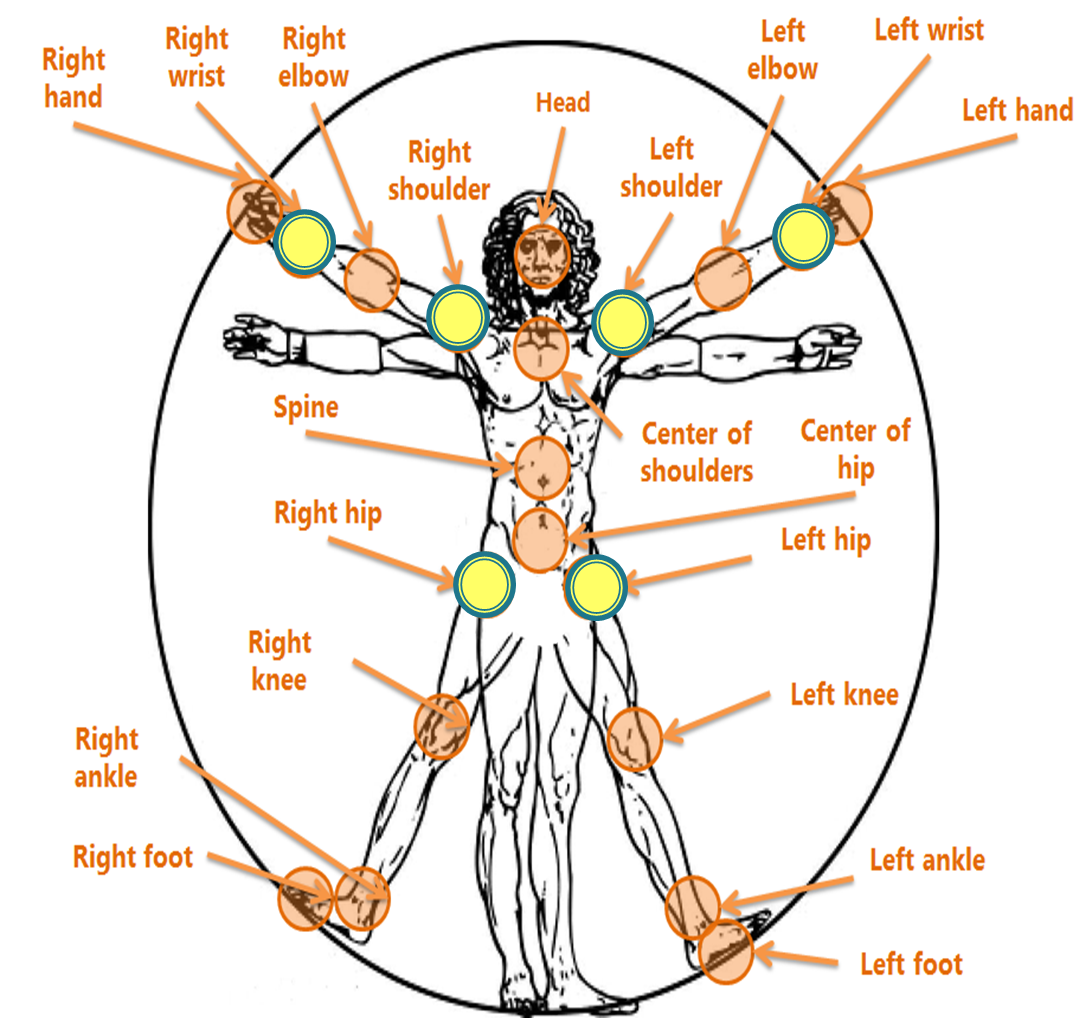
\includegraphics[height=2.6 in]{img/articulacoes-sel.png}
			%\caption{Modificações no Jogo ao Longo das Fases de Desenvolvimento~\cite{fullerton2008game}}
  \end{block}
\end{frame}

\begin{frame}{Movimento Angular}
  \begin{block}{Movimento de Abdução e Adução do Braço ~\cite{mcginnis2013biomechanics}}
      \center 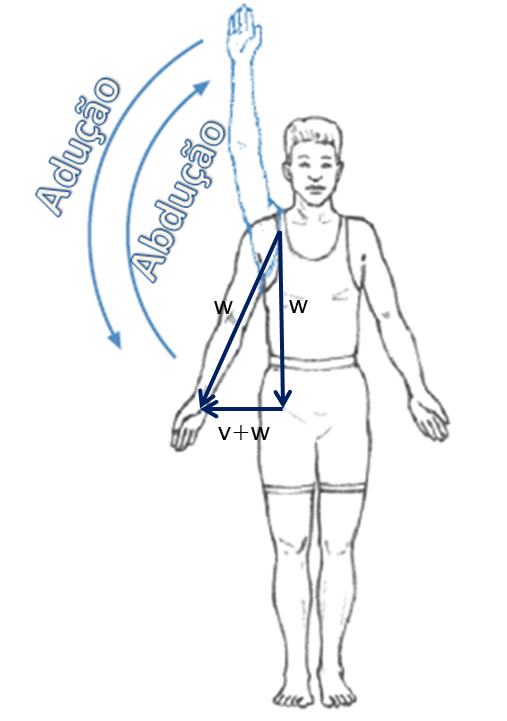
\includegraphics[width=4cm]{img/abducao-angulo.png}
			%\caption{Modificações no Jogo ao Longo das Fases de Desenvolvimento~\cite{fullerton2008game}}
  \end{block}
\end{frame}

\begin{frame}{Mecanismo de Identificação de Sintomas Motores}
  %\begin{block}{}
      \center 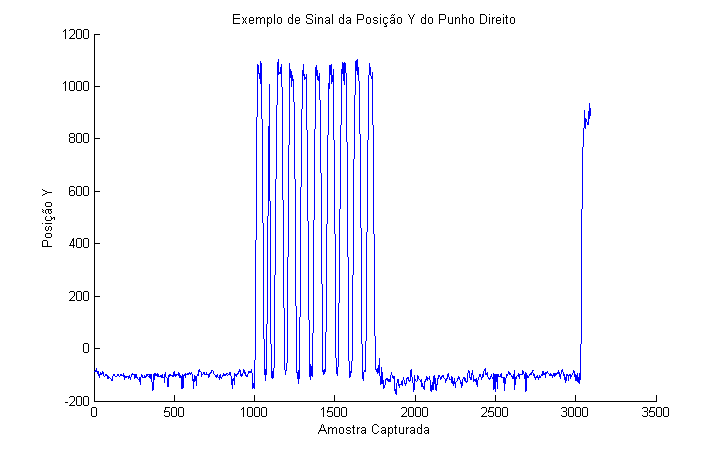
\includegraphics[height=3 in]{img/exsinalposicaoypunhodireito.png}
			%\caption{Modificações no Jogo ao Longo das Fases de Desenvolvimento~\cite{fullerton2008game}}
  %\end{block}
\end{frame}

\begin{frame}{Técnicas de Picos e Vales do Sinal}
  %\begin{block}{}
      \center 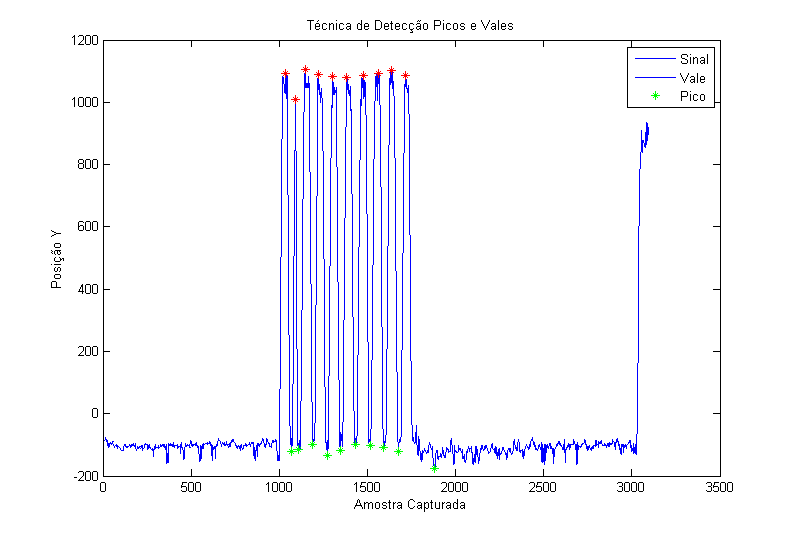
\includegraphics[height=3 in]{img/deteccaopicosvales.png}
			%\caption{Modificações no Jogo ao Longo das Fases de Desenvolvimento~\cite{fullerton2008game}}
  %\end{block}
\end{frame}

\begin{frame}{Extração de Início e Fim dos Ciclos de Movimento}
  %\begin{block}{}
      \center 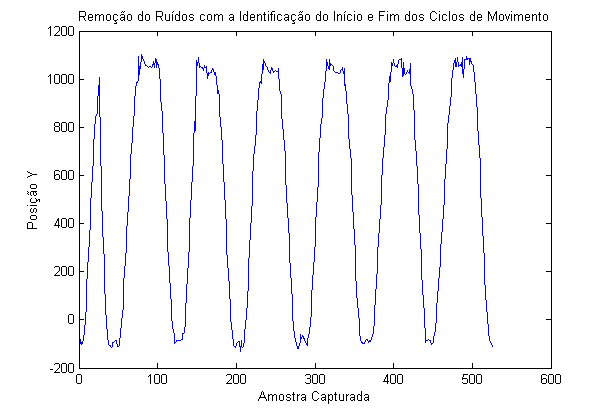
\includegraphics[height=3 in]{img/remocaoruidociclo.png}
			%\caption{Modificações no Jogo ao Longo das Fases de Desenvolvimento~\cite{fullerton2008game}}
  %\end{block}
\end{frame}


%\begin{frame}
   %\frametitle{Cálculo do Ângulo Relativo de Abdução e Adução do Braço}
   %\begin{block}{Produto Escalar}
   %
   %\begin{columns}[c]
     %\begin{column}{0.5\linewidth}
           %\begin{itemize}
           %\item O produto escalar é uma operação entre dois vetores cujo resultado é um escalar;
					 %\item O produto escalar é o ângulo de $ \theta$ formado entre os vetores $ v $ e $ w $;					 
           %\end{itemize}
				%%	\item \begin{math} cos(\theta) = (v . w) /  (||v|| ||w||) \end{math}
     %\end{column}
%
     %\begin{column}{0.5\linewidth}
				%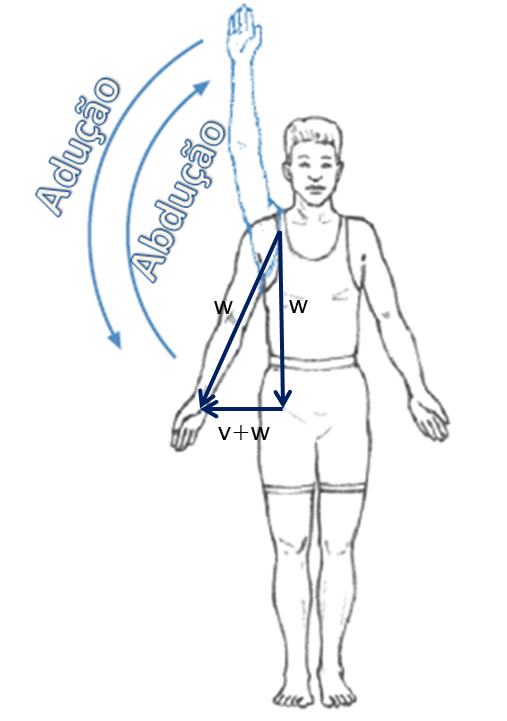
\includegraphics[width=4cm]{img/abducao-angulo.png}
    %\end{column}
%\end{columns}
%\end{block}
%\end{frame}


\begin{frame}{Cálculo da Velocidade Angular do Movimento de Abdução e Adução}
  %\begin{block}{}
      \center 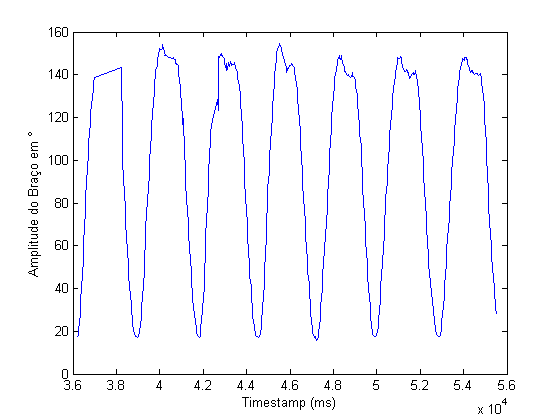
\includegraphics[height=2.8 in]{img/amplitude-braco.png}
			%\caption{Modificações no Jogo ao Longo das Fases de Desenvolvimento~\cite{fullerton2008game}}
  %\end{block}
\end{frame}

\begin{frame}{Filtragem de Dados: Remoção de Ciclos Incompletos}
   \begin{block}{}
   
   \begin{columns}[c]
     \begin{column}{0.5\linewidth}
				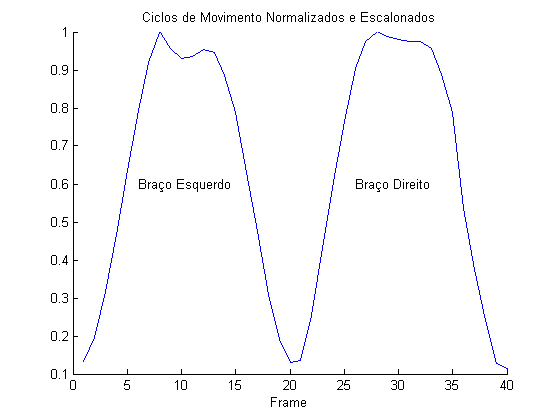
\includegraphics[width=5.5cm]{img/ciclonormalizadoescalonado.png}
     \end{column}

     \begin{column}{0.55\linewidth}
				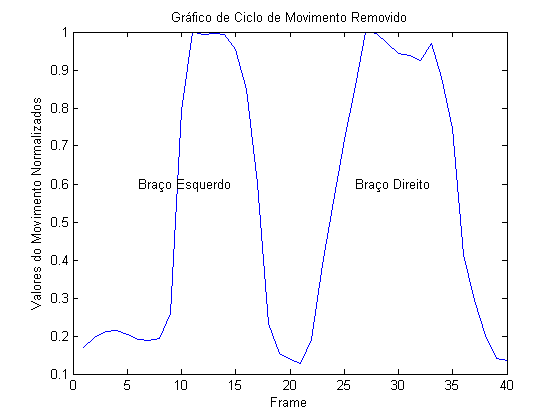
\includegraphics[width=5.5cm]{img/ciclomovimentoremovido.png}
    \end{column}
\end{columns}
\end{block}
\end{frame}

\begin{frame}{Classificador de Dados}
\begin{block}{}
			O classificador de dados, é utilizado na abordagem para identificar de possíveis usuários com problemas motores. Desta forma, o classificador irá auxiliar o profissional de saúde no acompanhamento de seus pacientes.
\end{block}
\end{frame}

%\subsection{Aprendizagem de Máquina Supervisionada}
\begin{frame}
   \frametitle{Máquina de Vetor de Suporte (SVM)}
   \begin{block}{}
   
   \begin{columns}[c]
     \begin{column}{0.5\linewidth}
			 \begin{itemize}
				\item Uma SVM utiliza vetores de separação através de uma técnica de hiperplano de separação ótima.

				\item Formalmente, classificadores que separam os dados por meio de um hiperplano utilizam um discriminante linear~\ref{eq:hiperplano}.
			\end{itemize}

			\begin{equation}
			f(x)=w^Tx+b
			\label{eq:hiperplano}
			\end{equation}.
     \end{column}

     \begin{column}{0.5\linewidth}
				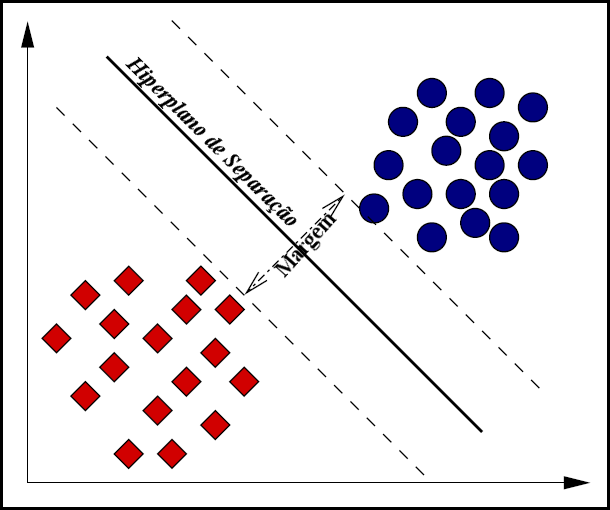
\includegraphics[width=4cm]{img/svmhyperplane.png}
    \end{column}
\end{columns}
\end{block}
\end{frame}

\begin{frame}{Visualização do Vetor Médio do Movimento de Abdução e Adução do Braço}
  %\begin{block}{}
      \center 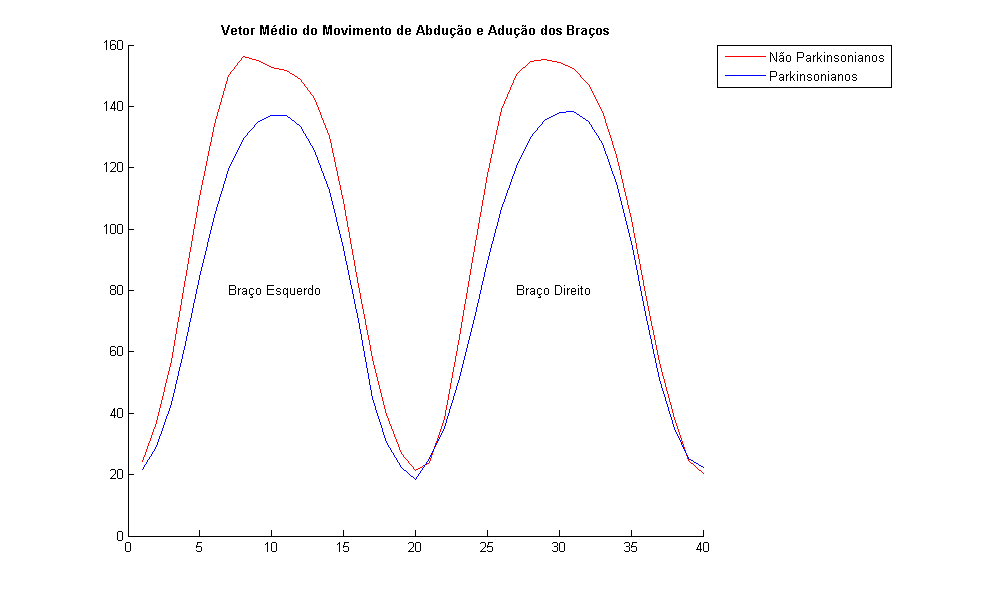
\includegraphics[height=2.6 in]{img/vetormedioaducao.png}
			%\caption{Modificações no Jogo ao Longo das Fases de Desenvolvimento~\cite{fullerton2008game}}
  %\end{block}
\end{frame}

%\subsection{Visualização}
\begin{frame}{Ciclos de Movimento de Abdução e Adução do Braço}
  %\begin{block}{}
      \center 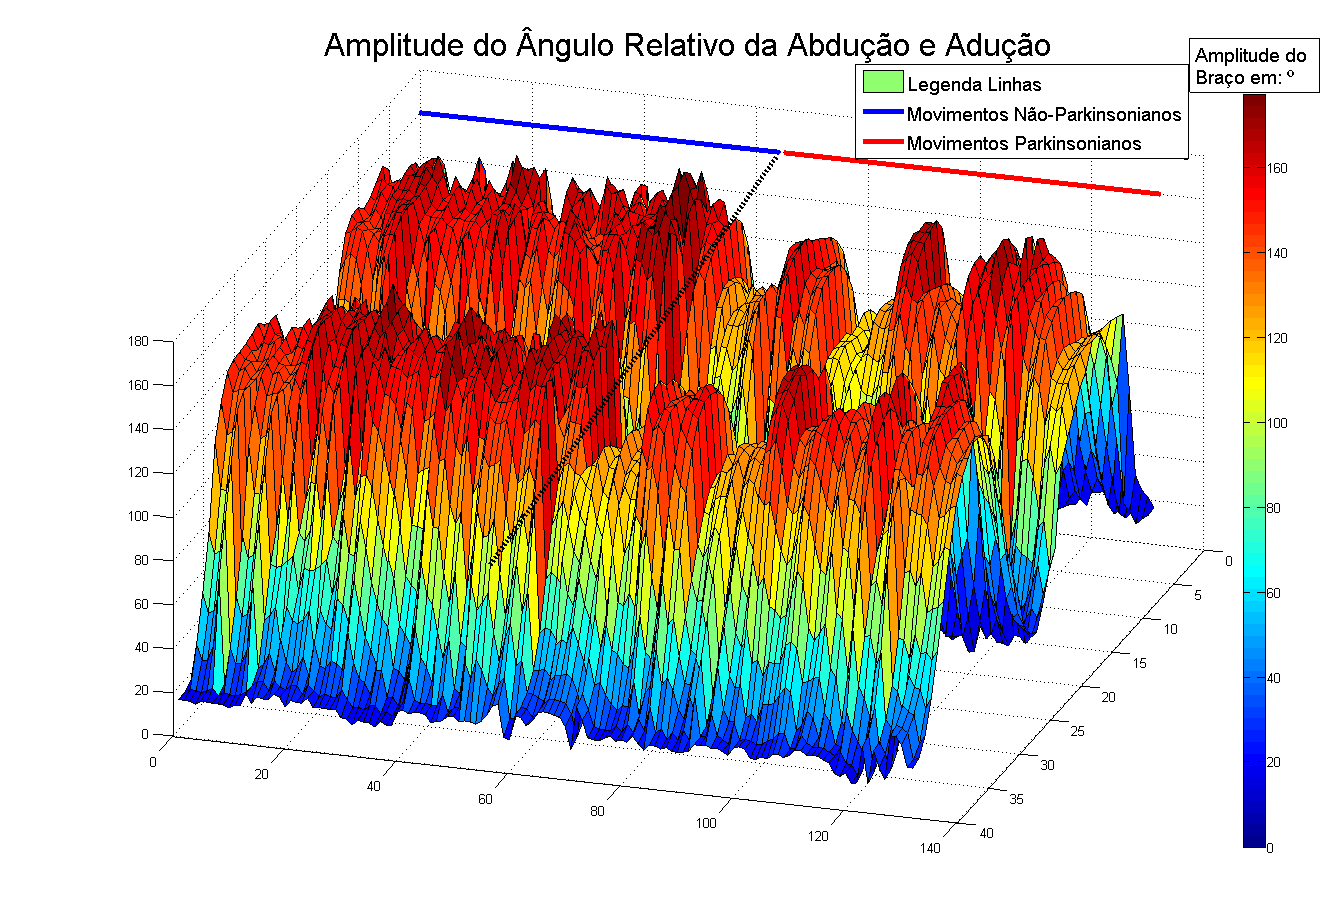
\includegraphics[height=3 in]{img/ciclosmovimentokinnect-2.png}
			%\caption{Modificações no Jogo ao Longo das Fases de Desenvolvimento~\cite{fullerton2008game}}
  %\end{block}
\end{frame}


\begin{frame}{Visualização das Características do Movimento}
  \begin{block}{}
      \center 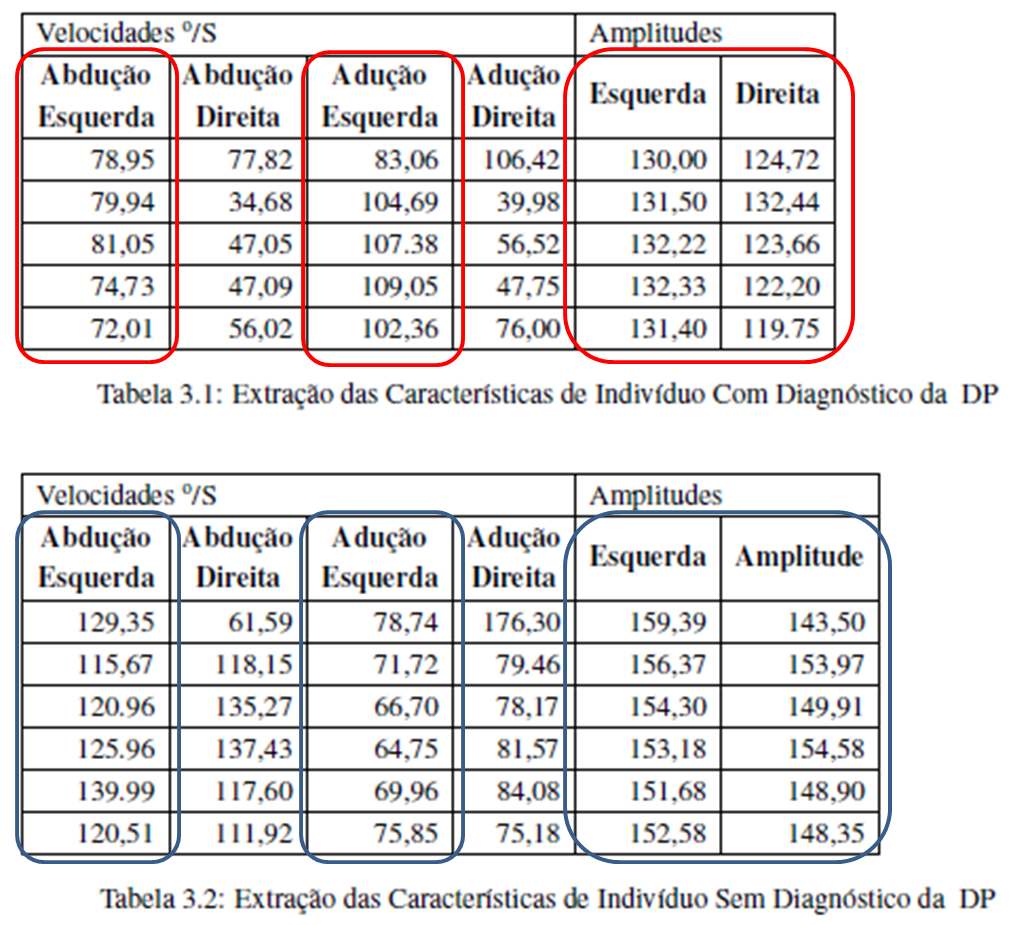
\includegraphics[height=2.8 in]{img/caracteristicas-tabela.png}
			%\caption{Modificações no Jogo ao Longo das Fases de Desenvolvimento~\cite{fullerton2008game}}
  \end{block}
\end{frame}

\section{Experimentos}
\subsection{}
%\subsection{Estudo Analítico de Caso-Controle}
\begin{frame}{Estudo Analítico de Caso-Controle: Identificação da Bradicinesia} 
    \begin{block}{Objetivo da Pesquisa}<1->
      Validar a Hipótese \textbf{H2}: É possível capturar dados motores por meio de sensores de movimento utilizados em jogos eletrônicos. Esses dados auxiliam no companhamento de doenças  com comprometimento motor.

    \end{block}
		\begin{block}{Coleta de Dados}<2->
			\begin{itemize}
				\item Protocolo de pesquisa submetido aprovado junto ao CEP da UFCG (\textbf{CAAE: 14408213.9.1001.5182})
				\item Coleta realizada nas instituições:
					\begin{enumerate}
						\item Hospital Universitário da UFAL;
						\item Fundação Pestalozzi;
						\item Clínica Fisioterapia do CESMAC;
						\item Instituto Federal de Alagoas;
						\item Universidade Federal de Campina Grande.
					\end{enumerate}				
			\end{itemize}
    \end{block}
\end{frame}

\begin{frame}{Amostra} 
    \begin{block}{}
			\begin{itemize}
				\item A técnica de amostragem utilizada para seleção, foi por conveniência, composta por:
				\begin{enumerate}
					\item 15 indivíduos portadores de DP;
					\item 12 sem o diagnostico, como grupo controle.
				\end{enumerate}
					\item No grupo de portadores de DP, foram inclusos indivíduos até o Estágio 3 (Doença bilateral leve a moderada com alguma instabilidade postural e capacidade para viver independente), segundo a UPDRS.
				\end{itemize}
    \end{block}
\end{frame}

\begin{frame}{Coleta dos Dados Utilizando o Jogo: \textit{Catch the Spheres}}
  %\begin{block}{}
      \center 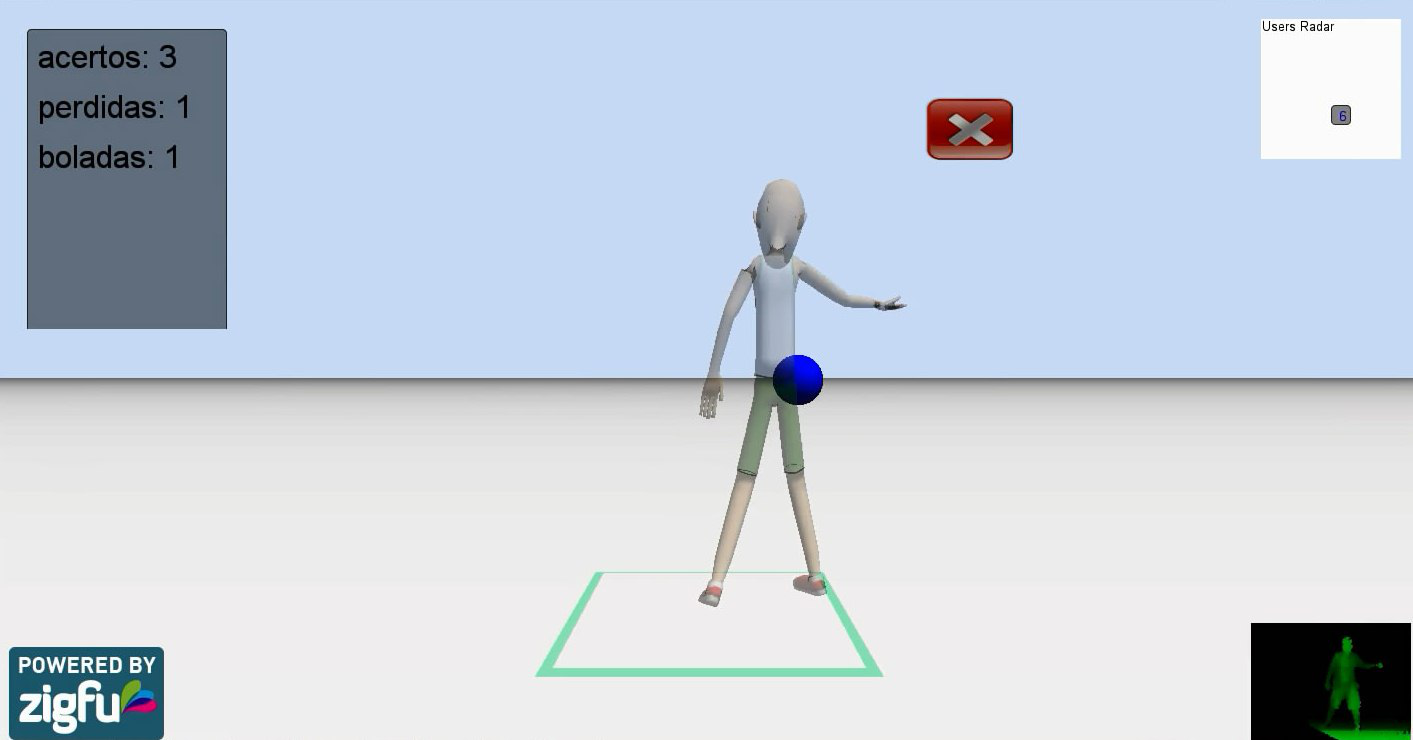
\includegraphics[height=2.2 in]{img/catch-the-spheres.png}
			%\caption{Modificações no Jogo ao Longo das Fases de Desenvolvimento~\cite{fullerton2008game}}
  %\end{block}
\end{frame}

\begin{frame}{Processo de Coleta de Dados}
   \begin{block}{}   
   \begin{columns}[c]
     \begin{column}{0.5\linewidth}
				\begin{itemize}[<+->]
					\item Voluntário se posiciona a 2m. do sensor de movimento;
					\item Voluntário inicia o jogo;
					\item Voluntário abduz e aduz o braço esquerdo, e depois o direito 10 vezes o mais rápido possível;
					\item Voluntário fecha o jogo.
				\end{itemize}
     \end{column}

     \begin{column}{0.55\linewidth}
				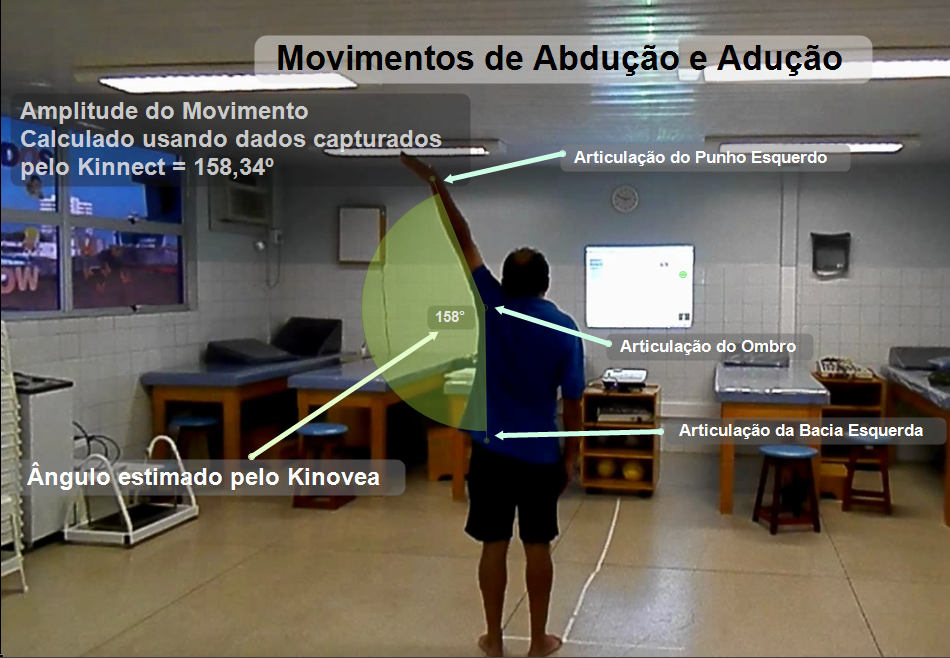
\includegraphics[width=5.5cm]{img/capturaducaokinnect.png}
    \end{column}
\end{columns}
\end{block}
\end{frame}



\begin{frame}{Processo de Coleta de Dados}
  %\begin{block}{}
      \center 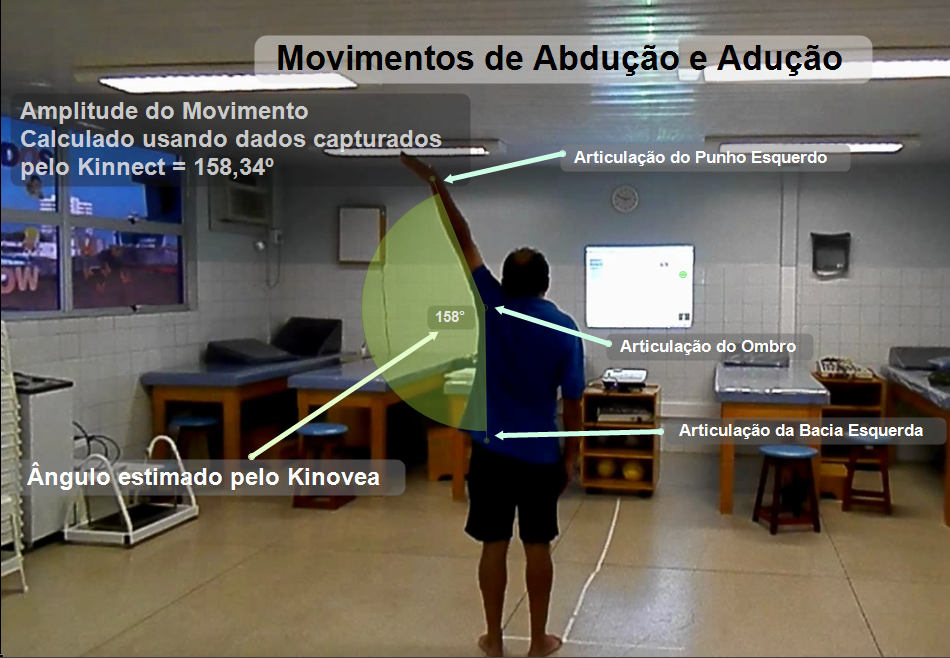
\includegraphics[height=2.6 in]{img/capturaducaokinnect.png}
			%\caption{Modificações no Jogo ao Longo das Fases de Desenvolvimento~\cite{fullerton2008game}}
  %\end{block}
\end{frame}

\begin{frame}{Características Extraídas do Movimento}
	\begin{block}{}
		\begin{itemize}[<+->]
			\item	Ciclo de movimento, normalizado e escalonado em 20 amostras;
			\item	amplitude do movimento de abdução do braço esquerdo e direito;
			\item	velocidade angular de abdução dos braços esquerdo e direito;
			\item velocidade angular de adução do braço esquerdo e direito.
		\end{itemize}
	\end{block}
\end{frame}

\begin{frame}{Classificação dos Dados}
	\begin{block}{}
		\begin{itemize}[<+->]
			\item	Com os dados coletados, realizou-se uma classificação usando SVM com núcleo linear e \textit{bias} de 0,10.
			\item	O resultado com o núcleo linear foi o mais expressivo ante o Polinomial, Radial e MLP.
		\end{itemize}
	\end{block}
\end{frame}

\begin{frame}{Matriz de Confusão}
	\begin{block}{Resultado da Matriz de Confusão do Estudo Analítico Caso-Controle Usando SVM Linear}
\begin{table}[!htbp]
		\label{table:resultadomatrizconfusaosvm}
		\centering
		\begin{tabular}{l|c|c|}
		\cline{2-3}
		\multicolumn{1}{c}{}                         & \multicolumn{2}{|c|}{\textit{\textbf{Classe Preditiva}}} \\ \cline{2-3} 
																								 & \textbf{Parkinson}      & \textbf{Não-Parkinson}         \\ \hline
		\multicolumn{1}{|l|}{\textbf{Parkinson}} & 12       & 3           \\ \hline
		\multicolumn{1}{|l|}{\textbf{Não Parkinson}}     & 2           & 10     \\ \hline
		\end{tabular}
\end{table}
	\end{block}
\end{frame}

\begin{frame}
   \frametitle{Métricas da Classificação}
   \begin{block}{}
   		\begin{table}[!htbp]
				\label{table:metricasmatrizconfusao}
				\centering
				\begin{tabular}{|l|r|}
				\hline
				\multicolumn{2}{|l|}{\textbf{Métricas}} \\ \hline
				\textbf{TpRate}                    & 80,00$\%$\                 \\ \hline
				\textbf{FpRate}                    & 16,67$\%$\                \\ \hline
				\textbf{Precision}                 & 85,71$\%$\                \\ \hline
				\textbf{Accuracy}                  & 81,48$\%$\                \\ \hline
				\textbf{F-Measure}                 & 82,76$\%$\                \\ \hline
				\end{tabular}
				\end{table}
	\end{block}
     \begin{block}{}
				\begin{description}
				\item [\textit{TpRate}]: taxa de acerto obtido;
				\item [\textit{FpRate}]: taxa de falso alarme obtido;
				\item [\textit{Precision}]: taxa de acerto de uma instância em determinada classe;
				\item [\textit{Accuracy}]: taxa de acerto de todo o classificador;
				\item [\textit{F-Measure}]: análise de classificador binário que mede a acurácia.
				\end{description}
    \end{block}
\end{frame}

\begin{frame}{Limitações do Método}
	\begin{block}{}
	A aprendizagem estatística deste trabalho é apenas um indicador, o qual necessita da interpretação do profissional de saúde.
	\end{block}
  \begin{block}{}
      \center 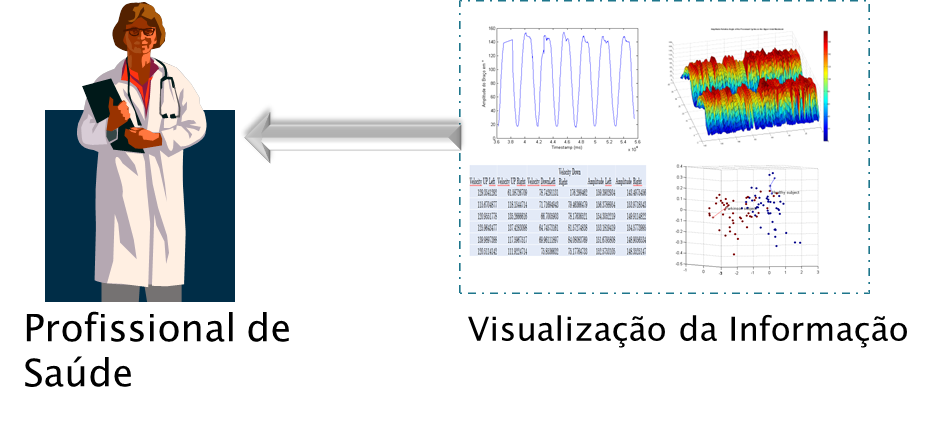
\includegraphics[height=1 in]{img/visualizacaomedico.png}
			%\caption{Modificações no Jogo ao Longo das Fases de Desenvolvimento~\cite{fullerton2008game}}
  \end{block}
\end{frame}

%\section{Outros Experimentos}
%\subsection{Identificação de Tremor}
\begin{frame}{Outros Experimentos}
	\begin{block}{Uso de Jogo em \textit{Smartphone} Para Detecção de Tremor}
	\center 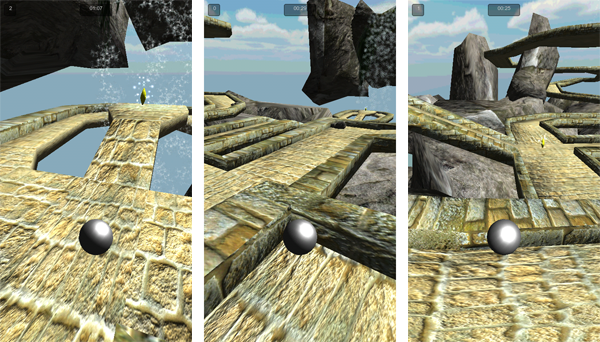
\includegraphics[height=1 in]{img/pinball_world.png}
	\end{block}
	\begin{block}{Insucesso na Quantificação}
			\begin{itemize}[<+->]
			\item Tremor da DP é de repouso.
			\item Indivíduos quando utilizavam o jogo reduziam drasticamente o sintoma.
			\item Como os dados não seriam satisfatórios, logo a coleta tornou-se inviável.
		\end{itemize}
	\end{block}
\end{frame}


%\subsection{Análise da Marcha}
\begin{frame}{Análise da Marcha por Base de Dados Pública (\textit{Parkinson Disease}~\cite{physionet}}
  \begin{block}{Objetivo do Estudo}
      \begin{itemize}[<+->]
				\item Aumentar o número de indivíduos da amostra;
						\begin{itemize}
							\item 50 Indivíduos Parkinsonianos;
							\item 50 Indivíduos Grupo Controle.
						\end{itemize}
				\item estudo de um movimento característico da doença;
				\item preservar a integridade física dos indivíduos;
				\item comparar os resultados obtidos.
			\end{itemize}
			%\caption{Modificações no Jogo ao Longo das Fases de Desenvolvimento~\cite{fullerton2008game}}
  \end{block}
\end{frame}

\begin{frame}{Sensor de Captura da FVRS \textit{Ultraflex Computer Dyno Graphy}}
  %\begin{block}{}
      \center 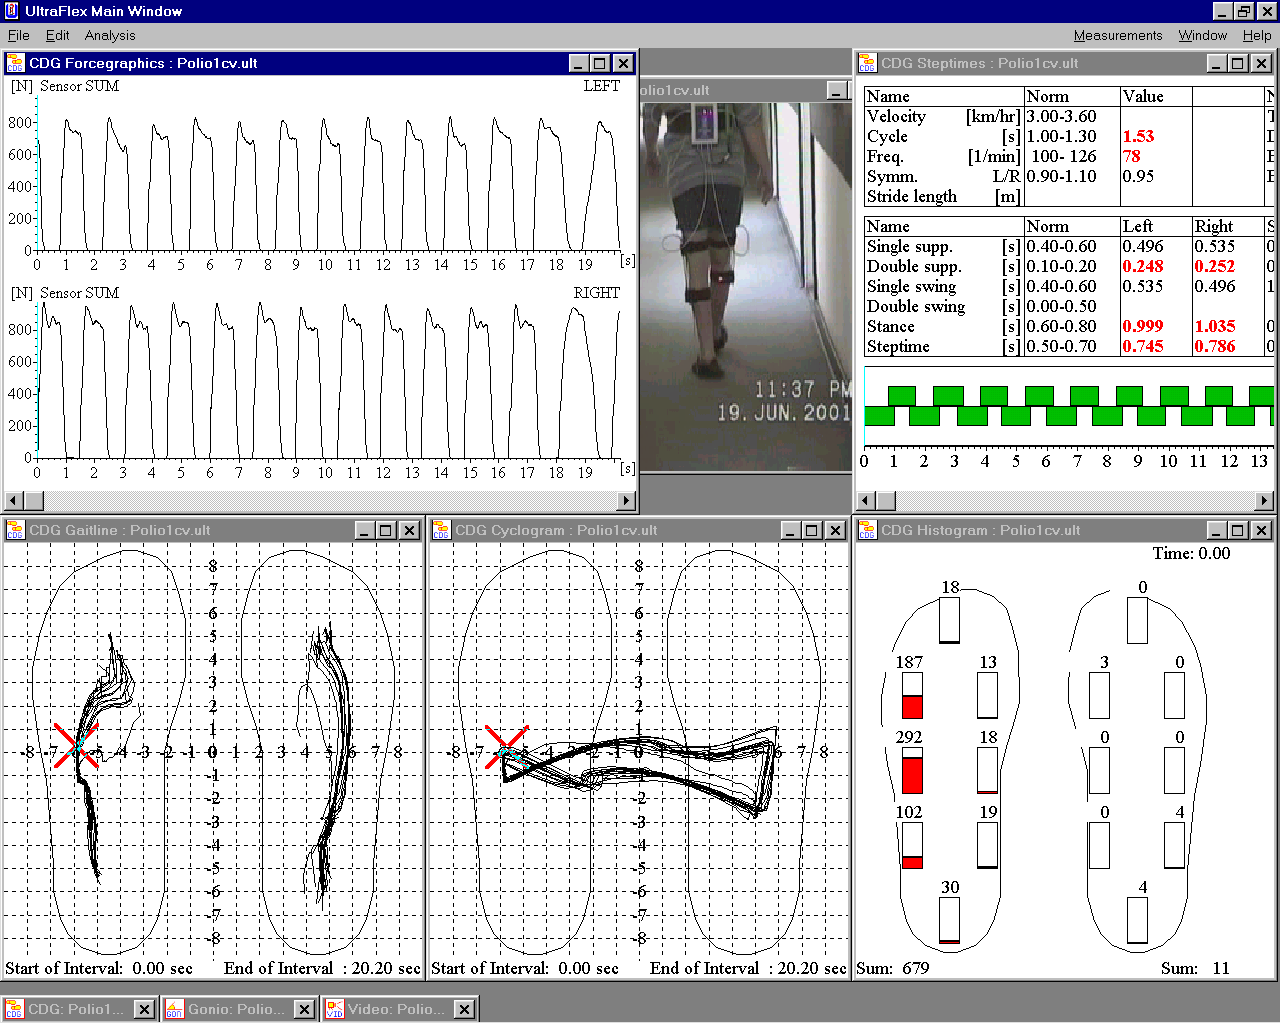
\includegraphics[height=2.8 in]{img/ultraflexdinografia.png}
			%\caption{Modificações no Jogo ao Longo das Fases de Desenvolvimento~\cite{fullerton2008game}}
  %\end{block}
\end{frame}

\begin{frame}{Análise da Marcha~\cite{neumann2012cinesiologia}}
  %\begin{block}{}
      \center 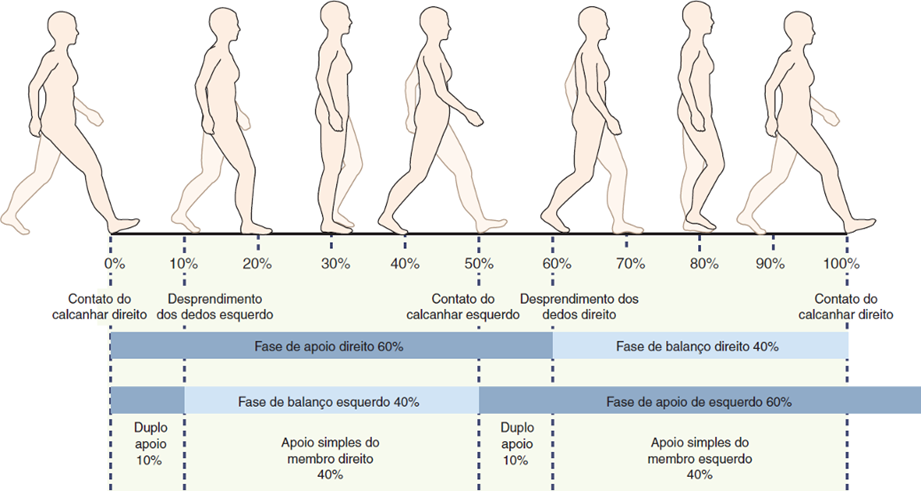
\includegraphics[height=2.2 in]{img/analisemarcha.png}
			%\caption{Modificações no Jogo ao Longo das Fases de Desenvolvimento~\cite{fullerton2008game}}
  %\end{block}
\end{frame}







\begin{frame}{Classificador: Análise de Componentes Principais (PCA)}
\begin{block}{}
			A PCA consiste em aplicar uma transformação linear nos dados de modo que o resultado desta transformação demonstre suas componentes mais relevantes ~\cite{smith2002}.
\end{block}

\begin{block}{Passos Para Execução:}
	\begin{enumerate}[<+->]
		\item Obter dados;
		\item subtrair a média;
		\item calcular a matriz de covariância;
		\item calcular autovalores e autovetores da matriz de covariância;
		\item escolher os componentes e formar os vetores de características;
		\item projetar no autoespaço;
		\item identificar indivíduo mais próximo por distância euclidiana.
	\end{enumerate}			
\end{block}
\end{frame}

\begin{frame}{Vetor Médio dos Ciclos da Marcha}
  %\begin{block}{}
      \center 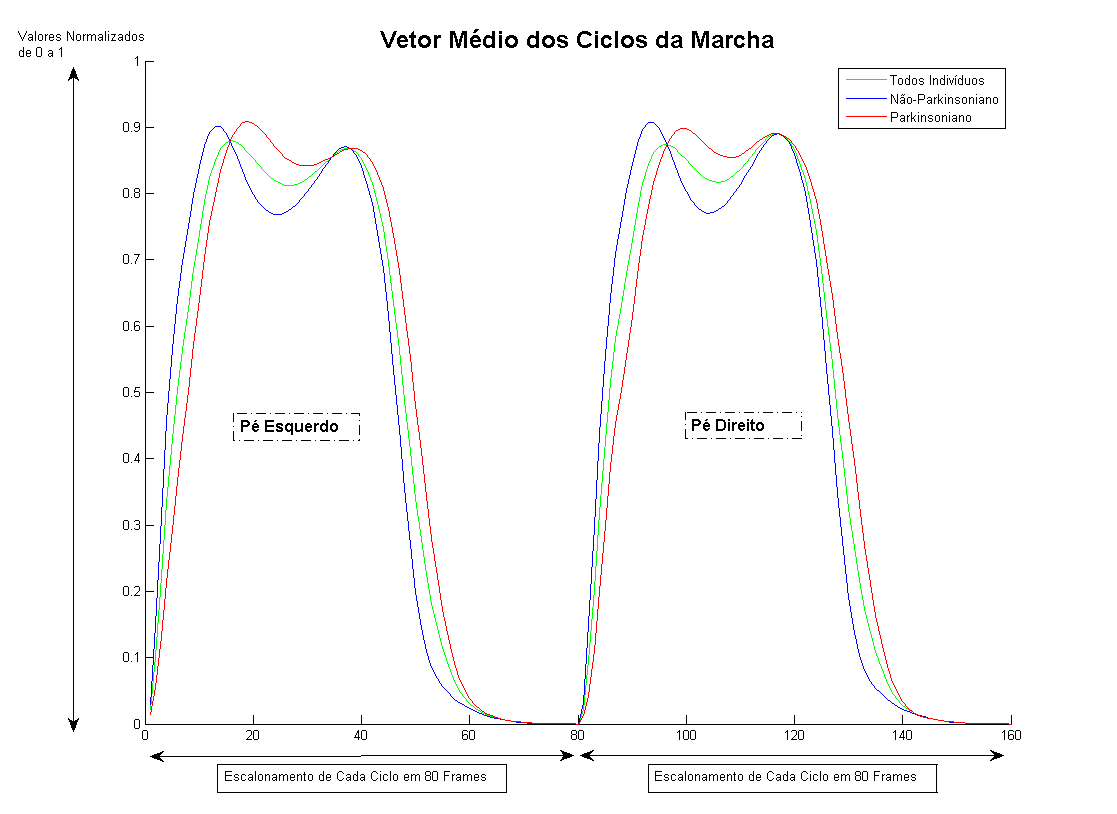
\includegraphics[height=2.6 in]{img/vetormediociclosdamarcha.png}
			%\caption{Modificações no Jogo ao Longo das Fases de Desenvolvimento~\cite{fullerton2008game}}
  %\end{block}
\end{frame}

\begin{frame}{Projeção dos Indivíduos no Autoespaço}
  %\begin{block}{}
      \center 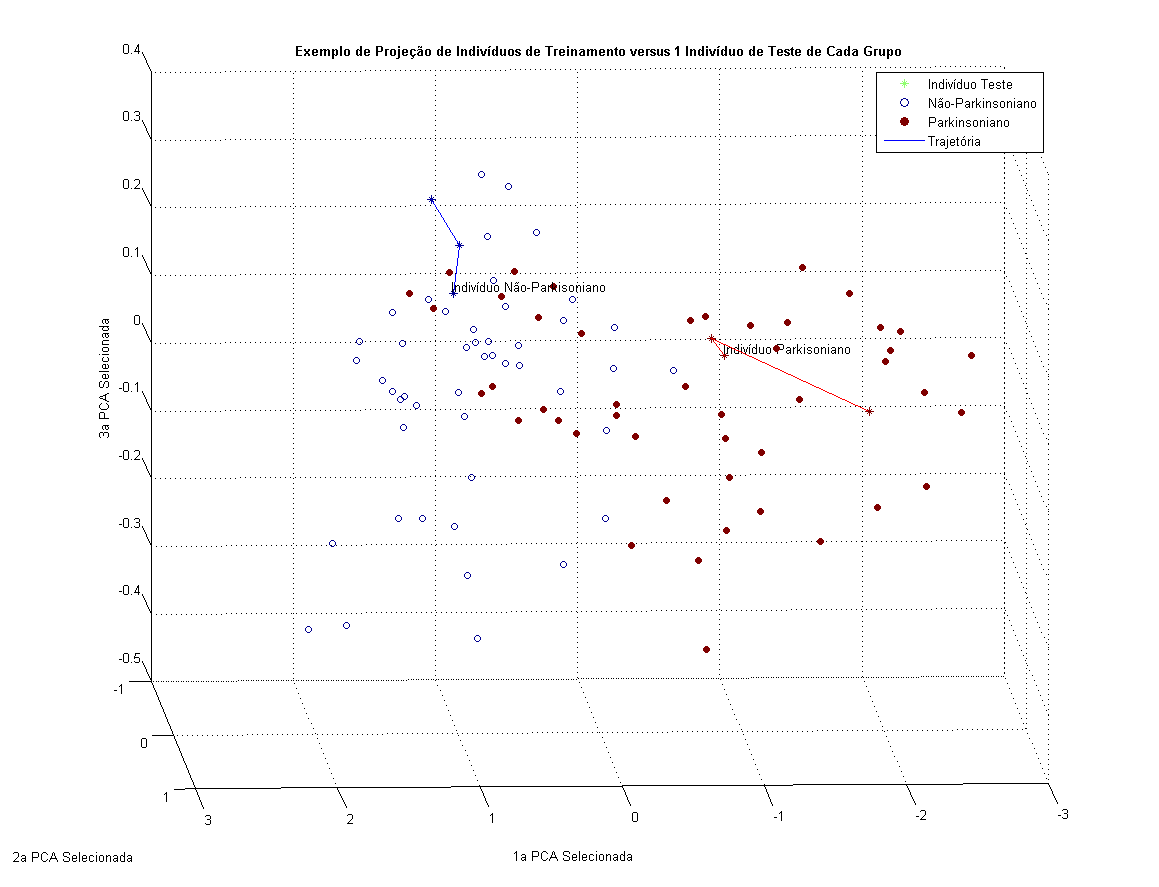
\includegraphics[height=2.6 in]{img/projecao-pca-parkinson-healthy.png}
			%\caption{Modificações no Jogo ao Longo das Fases de Desenvolvimento~\cite{fullerton2008game}}
  %\end{block}
\end{frame}

\begin{frame}{Resultado da Classificação}
   \begin{block}{PCA com validação cruzada com a repetição de 10 vezes o 10-K-Fold}   
   \begin{columns}[c]
     \begin{column}{0.5\linewidth}
				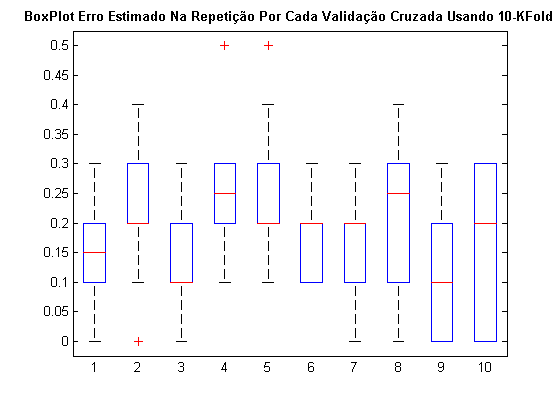
\includegraphics[width=5cm]{img/boxplot-eigengaits-parkinsondatabase-error-kfold.png}
     \end{column}

     \begin{column}{0.5\linewidth}
				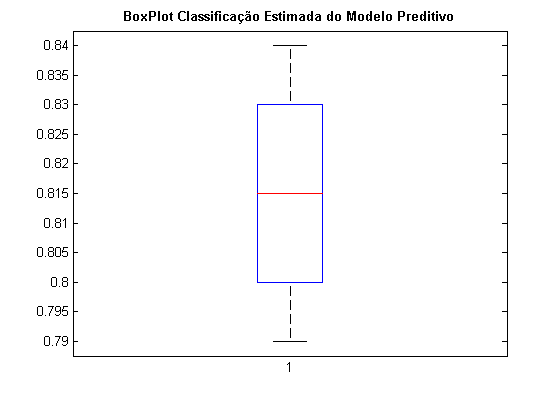
\includegraphics[width=5cm]{img/boxplot-eigengaits-parkinsondatabase.png}
    \end{column}
\end{columns}
\end{block}
\end{frame}

\begin{frame}{Matriz de Confusão}
	\begin{block}{Resultado da Matriz de Confusão da PCA na Base de Dados \textit{Parkinson Disease}}
\begin{table}[!htbp]
\label{table:resultadomatrizconfusaopca}
\centering
\begin{tabular}{l|c|c|}
\cline{2-3}
\multicolumn{1}{c}{}                         & \multicolumn{2}{|c|}{\textit{\textbf{Classe Preditiva}}} \\ \cline{2-3} 
                                             & \textbf{Parkinson}      & \textbf{Não-Parkinson}         \\ \hline
\multicolumn{1}{|l|}{\textbf{Parkinson}} & 429       & 71           \\ \hline
\multicolumn{1}{|l|}{\textbf{Não Parkinson}}     & 114           & 386     \\ \hline
\end{tabular}
\end{table}
	\end{block}
\end{frame}


\begin{frame}
   \frametitle{Validação Hipótese H2 - Matriz Confusão (Marcha-PCA e Movimento Adução-SVM)}
    %\begin{block}{PCA - Base de Dados \textit{Parkinson Disease}}
		\begin{block}{}
				\begin{table}
				\label{table:metricasmatrizconfusaosvm}
				\centering
				\begin{tabular}{|l|r|}
				\hline
				\multicolumn{2}{|l|}{\textbf{Métricas - PCA Base de Dados}} \\ \hline
				\textbf{TpRate}                    & 85,80$\%$\                 \\ \hline
				\textbf{FpRate}                    & 22,80$\%$\                \\ \hline
				\textbf{Precision}                 & 79,01$\%$\                \\ \hline
				\textbf{Accuracy}                  & 81,50$\%$\                \\ \hline
				\textbf{F-Measure}                 & 82,26$\%$\                \\ \hline
				\end{tabular}
				\end{table}
    \end{block} 
	
	%\begin{block}{SVM - Estudo Analítico Caso Controle}
	\begin{block}{}
   		\begin{table}[!htbp]
				\label{table:metricasmatrizconfusao}
				\centering
				\begin{tabular}{|l|r|}
				\hline
				\multicolumn{2}{|l|}{\textbf{Métricas - SVM Caso-Controle}} \\ \hline
				\textbf{TpRate}                    & 80,00$\%$\                 \\ \hline
				\textbf{FpRate}                    & 16,67$\%$\                \\ \hline
				\textbf{Precision}                 & 85,71$\%$\                \\ \hline
				\textbf{Accuracy}                  & 81,48$\%$\                \\ \hline
				\textbf{F-Measure}                 & 82,76$\%$\                \\ \hline
				\end{tabular}
				\end{table}
	\end{block}

\end{frame}

\section{GQM}
\subsection{}
\begin{frame}{Análise GQM com Usuários} 
    \begin{block}{Objetivo da Pesquisa}
      Validar a Hipótese \textbf{H3}: É possível desenvolver um jogo que tenha mecanismos de captura de dados motores embutidos, e que permita monitorar e quantificar esses dados de maneira não-invasiva.
    \end{block}
		\begin{block}{Participantes}
		Foram entrevistados um total de 24 indivíduos das seguintes instituições:
			\begin{itemize}
				\item Universidade Federal de Campina Grande;
				\item Instituto Federal de Alagoas;
				\item Clínica de Fisioterapia do CESMAC;
				\item Fundação Pestalozzi.
			\end{itemize}
    \end{block}
\end{frame} 

\begin{frame}{Questões da Pesquisa} 
    \begin{block}{}
			\begin{enumerate}
				\item Se o usuário integraria a abordagem GAHME à sua rotina diária.
				\item Se a segurança com a integridade física está de acordo com a faixa etária do usuário.
			\end{enumerate}
    \end{block}
\end{frame}

\begin{frame}{Integrar a Abordagem à Rotina Diária} 
    \begin{block}{Métrica 1.1: Escala de Diversão do Jogo}
			\center 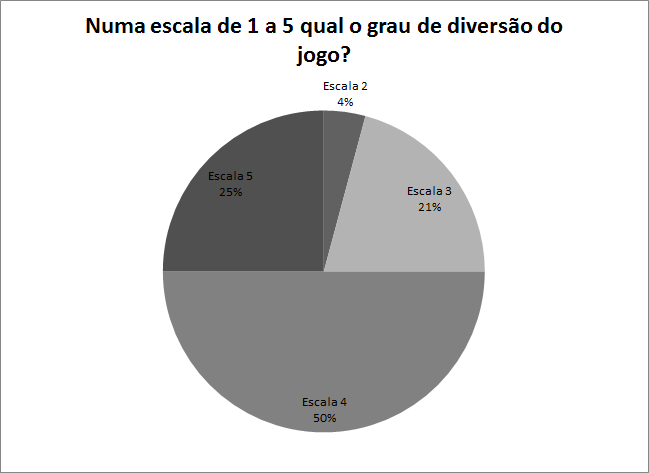
\includegraphics[height=2.6 in]{img/chart_1-.png}
    \end{block}
\end{frame}

\begin{frame}{Integrar a Abordagem à Rotina Diária} 
    \begin{block}{Métrica 1.3: Integrar o Jogo À Rotina Diária}
			\center 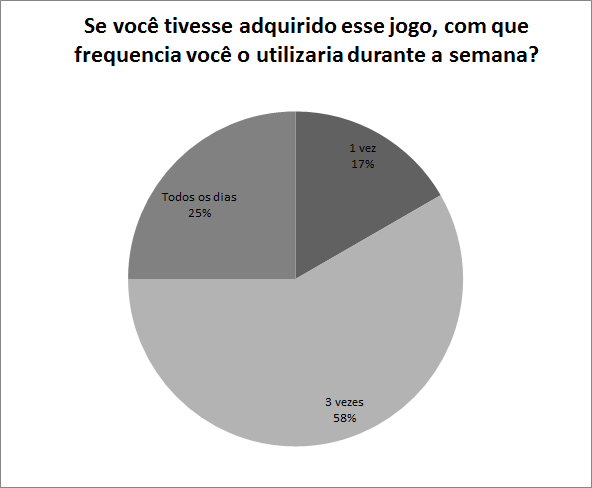
\includegraphics[height=2.6 in]{img/chart_3-.png}
    \end{block}
\end{frame}

\begin{frame}{Integrar a Abordagem à Rotina Diária} 
    \begin{block}{}
			\center 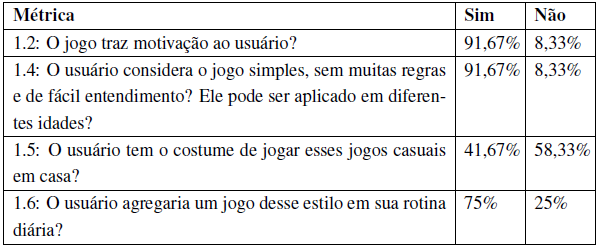
\includegraphics[height=1.4 in]{img/metricasq1.png}
    \end{block}
\end{frame}

\begin{frame}{Segurança à Integridade Física} 
    \begin{block}{Métrica 2.4: Faixa Etária do Jogo}
			\center 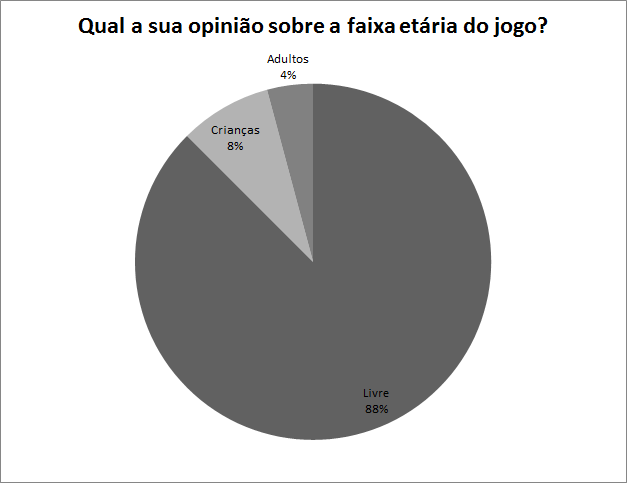
\includegraphics[height=2.6 in]{img/chart_10-.png}
    \end{block}
\end{frame}

\begin{frame}{Segurança à Integridade Física} 
    \begin{block}{}
			\center 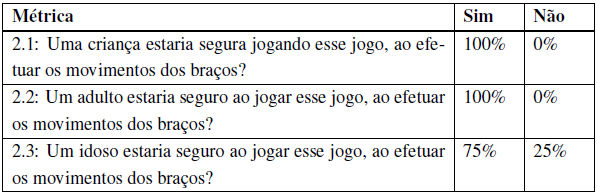
\includegraphics[height=1.4 in]{img/metricasq2.png}
    \end{block}
\end{frame}

%\begin{frame}{Segurança à Integridade Física} 
	%\begin{table}[h]
	%\centering
	%\begin{tabular}{|p{10cm}|p{1.2cm}|p{1.2cm}|}
	%\hline
	%\textbf{Métrica} & \textbf{Sim} & \textbf{Não} \\ \hline
%\begin{tabular}[c]{@{}c@{}}2.1: Uma criança estaria segura jogando esse\\ jogo, ao efetuar os movimentos dos braços e\\ das pernas ?\end{tabular}                              & 100\%                                              & 0\%                                                 \\ \hline
%\begin{tabular}[c]{@{}c@{}}2.2: Um adulto estaria seguro ao jogar esse\\ jogo, ao efetuar os movimentos dos braços\\ e das pernas ?\end{tabular}                               & 100\%                                              & 0\%                                                 \\ \hline
%\begin{tabular}[c]{@{}c@{}}2.3: Um idoso estaria seguro ao jogar esse jogo, ao efetuar os\\ movimentos dos braços e das pernas?\end{tabular}                                   & \multicolumn{1}{|l|}{75\%}                         & 0\%                                                 \\ \hline
%
	%\end{tabular}
	%\label{table:resultados_gqm}
	%\end{table}
%\end{frame}

%\section{Comparativo}
%\subsection{Análise da Marcha x Adução e Abdução do Braço}
%
%
%\section{GQM}
%
%\section{Estado Atual}

\section{Finalização}
\subsection{}
\begin{frame}{Publicação}
\begin{block}{}
Medeiros L., Fischer. R., Oliveira H., Silva L, and Perkusich A. \textbf{Monitoring parkinson
related gait disorder with eigengaits} - \textit{XX World Congress on Parkinson Disease and Related Disorders} - 2013.
\end{block}
\end{frame}

\begin{frame}{Finalização do Trabalho}
\begin{enumerate}[<+->]
	\item Realizar estudo de Regressão Linear nos Dados do estudo Caso-Controle (Ms-Kinnect);
	\item Realizar estudos de curva de aprendizagem nos Dados do estudo Caso-Controle;
	\item Refinar o processo de desenvolvimento para as fases de Construção e Pós-Validação;
	\item Analisar o motivo da ocorrência de 2 indivíduos de controle que foram classificados como Parkinsonianos.
\end{enumerate}
\end{frame}


%\subsection{Dúvidas}
\begin{frame}
  \begin{center}
  DÚVIDAS ?
  \end{center}
\end{frame}

%\subsection{Bibliografia}
%\bibliographystyle{alpha}
\bibliographystyle{authordate2}
%\bibliographystyle{plain} % estilo de bibliografia   plain,unsrt,alpha,abbrv.
%\bibliography{../../tex/bibtex/biblmm} % arquivos com as entradas bib.
\bibliography{biblmm} % arquivos com as entradas bib.

\end{document}
	